\documentclass{llncs}
%\documentclass{article}
\usepackage[utf8]{inputenc}
\usepackage{cite}
\usepackage{verbatim}
\usepackage{graphicx}
%\usepackage{wrapfig}
\usepackage{appendix}

\newcommand{\rdfterm}[1]{\texttt{#1}}
\newcommand{\pvalue}{\textit{p}-value}
\newcommand{\httph}[1]{\texttt{#1}}
\newcommand{\todo}[1]{\ensuremath{^{\textrm{\tiny{TODO}\normalsize}}}\footnote{\textbf{TODO:}~#1}}

\title{A survey of HTTP caching options on the open Web}
\author{Kjetil Kjernsmo\inst{1}}
\institute{Department of Informatics,
Postboks 1080 Blindern,
N-0316 Oslo, Norway \email{kjetil@kjernsmo.net}}

\subtitle{---Unpublished Working Draft, do not circulate---}


\begin{document}
\maketitle

\begin{abstract}
\end{abstract}

\section{Introduction}

Caching has been given a prominent place in the foundational documents
of the World Wide Web. Out of the 6 documents that make up the HTTP
1.1 standard, RFC7234 \cite{rfc7234} is entirely devoted to the topic,
and RFC7232 \cite{rfc7232} defines conditional requests, which is also
important when constructing caches. As the former notes:
\begin{quote} 
  The goal of caching in HTTP/1.1 is to significantly improve
  performance by reusing a prior response message to satisfy a current
  request.
\end{quote}
Furthermore, the Architecture of the World Wide Web
\cite{Jacobs:04:AWW} discusses caching throughout, and the definition
of the Representational State Transfer (REST) architectural style
\cite{Fielding_2000_Architectural-Styles} is partly motivated from the
requirement to implement efficient caching. We also note that caching
in the Internet infrastructure, through so-called Content Delivery
Networks, is both a large business area and something that could
provide great value to the Semantic Web community.

In spite of this, we have not seen it in widespread use in the
Semantic Web, and therefore we decided to conduct a survey to
investigate the actual compliance to RFC7234 and RFC7232. Our reasons
to do this include\todo{formulate as contributions?}
\begin{enumerate}
\item Understand the actual usage rather than rely on anecdotal
  conceptions.
\item Encourage the implementation of these mechanisms in Semantic Web
  infrastructure.
\item Point out future research directions.
\end{enumerate}

We note that caching is not only useful for long-living information
resources, even though that may be the most important. If a resource
is frequently requested, it may make sense to cache it even though it
may be fresh for only a very short period.

Caching may be deployed at several different levels: A HTTP cache may
be in a reverse proxy close to the server, in which case it may have
much in common with a conventional database cache. It may also be
anywhere between a server and a client, in which case it may be
shared, i.e. it may cache responses from several servers served to
several clients. Another example is an institutional forward proxy,
which are close to several users. Finally, the User Agent may
implement a private cache for its user at the client side.

Caching, as defined in RFC7234, requires that the server declares how
long into the future it expects the information resource in the
response to remain fresh, i.e. how long it is permissible to use
it. Based on this, the client need not contact the server at all to
reuse a cached response, but this requires a commitment from the
content provider. The standard also gives the client an opportunity to
heuristically determine a time to live. RFC7232, on the other hand,
defines a protocol for asking the server if the cached response is
still fresh using conditional requests. This doesn't burden the
content provider with the task of estimating the time to live
beforehand, but then, it must be able to answer if the resource has
changed less expensively than serving the entire response. These two
approaches can be combined, as a client may ask if a response is fresh
after it has expired.

In \cite{ldf1}, it was asserted that SPARQL query caching is only
possible on a per-query basis, but future research should challenge
this assumption. With this in mind, if reasoning is not involved, we
note that ontologies are not relevant to query answering since they
usually occur in bound terms. It is interesting to understand caching
when this is not the case. Moreover, many ontologies are maintained by
a small group of humans and change seldomly.\todo{not particularly clear}

Key contributions of this paper are:\todo{write}

\section{Related work}

We are not aware of any surveys of this type. Although the database
literature is rich with query cache literature, it is mostly relevant
to what would happen within the server or between the server and a
reverse proxy, which is opaque to the Internet, and therefore not of
our concern.

The \cite{dyldo2} Dynamic Linked Data Observatory (DyLDO)
performed, and continue to do so, of parts of the Linked Open Data
Cloud to determine dynamicity characteristics of Linked Data. Caching
is one of their motivations, but they have not published statistics on
HTTP headers.

Linked Data Fragments \cite{ldf1} claims to take advantage of caching
and contrasts this with the unavailability of SPARQL query caches, and
claims this is an architectural problem.

The implications of HTTP for query caches has been discussed by
\cite{kaseicache}. In \cite{sparqlproxy} the authors implemented a
reverse proxy that controlled the changes to the dataset, and
therefore could make sure the proxy had all the information needed to
determine freshness. We are interested in the situation where the
changes cannot be controlled.

A general caching approach is given in \cite{yang2011caching}.  In
\cite{umbrich2012hybrid}, the term caching was used in a different
sense than we do, they rather prefetch an entire dataset to a local
store and based on heuristics tried to determine which parts of the
query should be evaluated remotely and locally. \cite{lampo2011cache}
explored when caching had a positive effect on complex SPARQL queries.

In the broader Web literature, \cite{ager2010revisiting} analysed the
value of caching based anonymized traces of actual Web usage at a
major Internet Service Provider.

\section{Methodology}

We want to find information resources on the Web, and examine HTTP
headers that may allow caching. We record headers recommended by
current standards, as well as obsoleted and non-standard
headers. Additionally, we examine the triples in the returned
information resources to see if there is information there that may be
used to calculate heuristic freshness.

However, as the community has both spidered the Web as well as
recorded lists of relevant resources, we need not do that ourselves. 

The SPARQLES survey\cite{buil2013sparql} has recorded the availability
of SPARQL endpoints registered in the datahub.io portal, and found
that many of them have ceased to operate. We used their list of SPARQL
endpoints as of 2014-11-17, and filtered out those deemed unresponsive
by them. This resulted in a list of 312 endpoints.

To compile a list of Web ontologies, we first queried the Linked Open
Vocabularies (LOV) \cite{lov2} SPARQL endpoint
to retrieve all registered ontologies. Then, we took the full list of
URIs registered with prefix.cc. The assumption that they all identify
an ontology is clearly false, as we found that for example Tim
Berners-Lee's FOAF profile has a registered URI, but it is unlikely to
introduce significant bias.

To examine as many different implementations and hosts as possible, we
noted that the Billion Triple Challenge 2014 \cite{btc-2014} dataset
consisted of a 4~GTriple corpus of spidered Web data. To compile a
list of interesting candidates to further examine, we performed a
series of data reduction steps, manually inspecting the result between
each step. The details of this process is given in
Appendix~\ref{app:reduction}.

The end result of this process is a list of 3117 unique hosts, for
each several resources would be visited, some several times, as they
may host SPARQL Endpoints, ontologies, or other information resources,
by a spider detailed in Appendix~\ref{app:fetcher}, resulting in 7745
requests.

This results in an NQuads file per host, which is then loaded into a
Virtuoso-based SPARQL Endpoint for analysis by using the statistics
system R\cite{kn:r}.

\section{Analytics}

A\todo{Do I need details on how to compute the freshness lifetime?}

\subsection{Different server implementations}

First, we investigated whether certain servers provided better support
for caching than others. To do this, we formulated SPARQL queries to
examine the \httph{Server} headers of successful responses, with
optional clauses matching the standard-compliant computed freshness
time (which is the ideal) as well as whether the response had other
promising features that could assist caching, modification time,
certain predicates, etc.

For each unique \httph{Server} header, we found the ones where
\emph{all} responses had a freshness time or a promising feature. For
the former, this amounted to 22 servers, tabulated
in~\ref{tab:servers}. 70 servers always responded with promising
features. As we can see, apart from well-known Virtuoso and
Callimachus servers, as well as the Perl modules RDF::LinkedData and
RDF::Endpoint, which is partly developed by and runs on a server
operated by this author, most headers tells very little about the
RDF-specific parts of the underlying server implementation. A quick
inspection of all \httph{Server} headers confirmed that few reveal any
further detail.

% latex table generated in R 2.15.1 by xtable 1.5-6 package
% Mon Jan  5 11:27:35 2015
\begin{table}[ht]
  \caption{\httph{Server} headers for hosts that enabled a freshness
    lifetime to be computed for all requests.}\label{tab:servers}
\begin{center}
\begin{tabular}{rl}
  \hline
 & x \\ 
  \hline
1 & DFE/largefile \\ 
  2 & git\_frontend \\ 
  3 & nginx/1.3.9 \\ 
  4 & thin 1.6.0 codename Greek Yogurt \\ 
  5 & Oracle-Application-Server-10g/10.1.3.4.0 Oracle-HTTP-Server OracleAS-Web-Cache-10g/10.1.2.3.1 (N;ecid=72058133508068653,0) \\ 
  6 & Oracle-Application-Server-10g/10.1.3.4.0 Oracle-HTTP-Server OracleAS-Web-Cache-10g/10.1.2.3.1 (N;ecid=72057948824487974,0) \\ 
  7 & TwistedWeb/8.2.0 \\ 
  8 & RDF::Endpoint/0.07 \\ 
  9 & Jetty(6.1.26) \\ 
  10 & nginx/1.6.1 \\ 
  11 & Jigsaw/2.3.0-beta3 \\ 
  12 & Apache/2.2.9 (Win32) PHP/5.2.6 \\ 
  13 & Apache/2.4.10 (Unix) mod\_fcgid/2.3.9 \\ 
  14 &  \\ 
  15 & GFE/2.0 \\ 
  16 & RDF::LinkedData/0.70 \\ 
  17 & Apache/2.2.17 (Unix) mod\_wsgi/3.3 Python/2.6.6 \\ 
  18 & Virtuoso/07.10.3211 (Linux) i686-generic-linux-glibc212-64  VDB \\ 
  19 & Apache/2.2.24 (Unix) mod\_ssl/2.2.24 OpenSSL/0.9.8y \\ 
  20 & Apache/2.2.22 (Fedora) \\ 
  21 & INSEE \\ 
  22 & GitHub.com \\ 
   \hline
\end{tabular}
\end{center}
\end{table}

For a more systematic approach, we wish to test the hypothesis that
some servers are better configured to support caching than others. To
test this hypothesis, we create two so-called \emph{contigency
  tables}\cite{kn:bj}. This formalism is suited to see if the
distribution of  \httph{Server} headers are different for those implementations that
offer caching headers from those that don't. Intuitively, we expect
these distributions to be similar, ``long-tail'' distributions, i.e. a
handful of servers are used by a large number of projects, and then it
falls off rapidly, and so, some servers are used only by very
few. Likewise, it is only to be expected that only a few projects have
given caching enough attention, but that they account for the majority
of the support. The question is if the presence of caching headers is
merely a matter of proportion, or if there are some that have given it
more attention, but still is in relatively little use.

Using the statistics system R\cite{kn:r}, we use a statistical test,
namely Pearson's $\chi^2$ test with simulated \pvalue (based on 10000
replicates). The simulation is done using a Monte Carlo method to
compensate for the fact that many servers will not expose caching
headers at all, an issue that would otherwise violate the underlying
assumptions of the test.

In both the cases of standard-compliant freshness time and for the
other promising features, the test reports \pvalue = 0.0001. We can
conclude that it is highly likely that some servers are better at
exposing cache headers than others. Unfortunately, since most
\httph{Server} headers only report generic values, little can be
learnt about these implementations. We note, however, that DBPedia
exposes standards-compliant freshness time of 604800 seconds (i.e. 1
week) for both LOD and SPARQL endpoints.

\subsection{Other caching headers}

The two most important headers to control caching are \httph{Expires}
and \httph{Cache-Control}. As shown in Table~\ref{tab:headers}, there
are also others. We found \httph{Pragma} in 287 responses, but except
for two hosts, where they were superflous, they were only used to
prohibit caching. \httph{Surrogates} were not observed.

\subsection{Distribution of freshness time}

We obtained a successful response from a total 2965 information
resources, either with SPARQL results or RDF data. A successful
response is rather tightly defined, not only must there be a
successful HTTP response after redirects are resolved, the response must also
return a valid RDF media type (unless it is a SPARQL result) and the
RDF must parse into an RDF model.

Since web servers may be configured to instruct clients and proxies to
cache errors differently from successfully served requests, we should
first investigate whether we can simply use all cache headers in the
analysis, or if we should remove unsuccessful responses to avoid
introducing bias to the analysis of valid responses.

For a visual inspection, we may use a quantile-quantile plot to plot
the freshness lifetimes of successful responses versus requests that
failed for some reason. If the distribution of both variables are the
same, these points will lie on a straight line. In
Figure~\ref{fig:errorsqq}, we see successful responses vs. the most
common parse error, and it is clear that these are so different that
no further formal analysis is necessary, we must filter unsuccessful
requests in the following analysis.


\begin{figure}[ht!]
  \centerline{%
    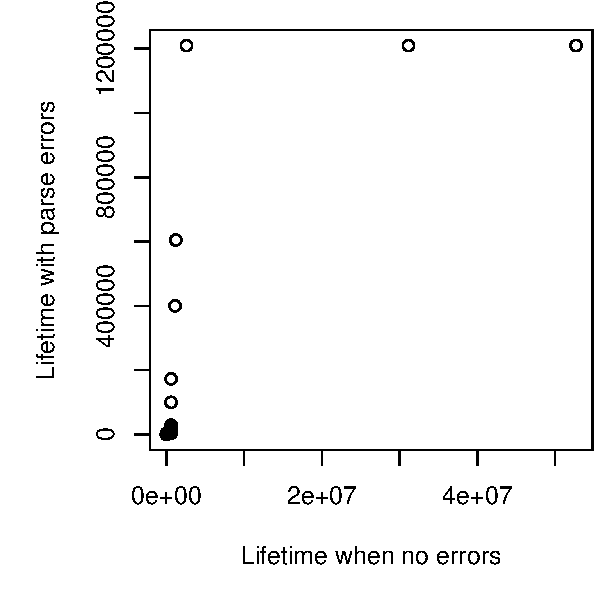
\includegraphics[width=.5\textwidth]{errorsqq.pdf}}
  \caption{A quantile-quantile plot of freshness lifetimes for
    standard compliant headers with and without errors.}
  \label{fig:errorsqq}
\end{figure}


\subsubsection{Standards-compliant caching headers}

Of these resources, 405 returned valid headers, but 114 did so to
\emph{prohibit} caching of the response, and 3 contained conflicting
headers, i.e. set an freshness lifetime, but also prohibited
caching. In most cases, \httph{Cache-Control} and \httph{Expires} both
occured, but the former is more common than the latter in the cases
where only one of them occur.  Additionally, 269 resources had a
\httph{Cache-Control} header to control other aspects of caching than
lifetime, i.e. to say that only private caches may use the response,
that the cache must be revalidated, or to prohibit caching.

Caching may also be prohibited by setting a non-positive freshness
lifetime. Common practice is to set the \httph{Expires} header to a
date far back in time, which has also been done in large parts of the
present dataset. For the following, we have set any non-positive
lifetime to 0, as that is semantically equivalent. With that, we
obtain the summary statistics in Table~\ref{tab:summaryhard}. 

\begin{table}[ht]
\begin{center}
\caption{Summary statistics for standards-compliant freshness lifetime}\label{tab:summaryhard}
\begin{tabular}{lr}
Min.   &       0   \\ 
1st Qu.&       0   \\ 
Median &     600   \\ 
Mean   &  583003   \\ 
3rd Qu.&  172800   \\ 
Max.   & 52702521   \\ 
   \hline
\end{tabular}
\end{center}
\end{table}

In Figure~\ref{fig:hardall}, there is a barplot where
the freshness lifetime is grouped in bins. We see that in these
categories, the most common is to prohibit caching. Nevertheless, many
also declare a standards compliant freshness lifetime in minutes to
days.

\begin{figure}[ht]
  \centerline{%
    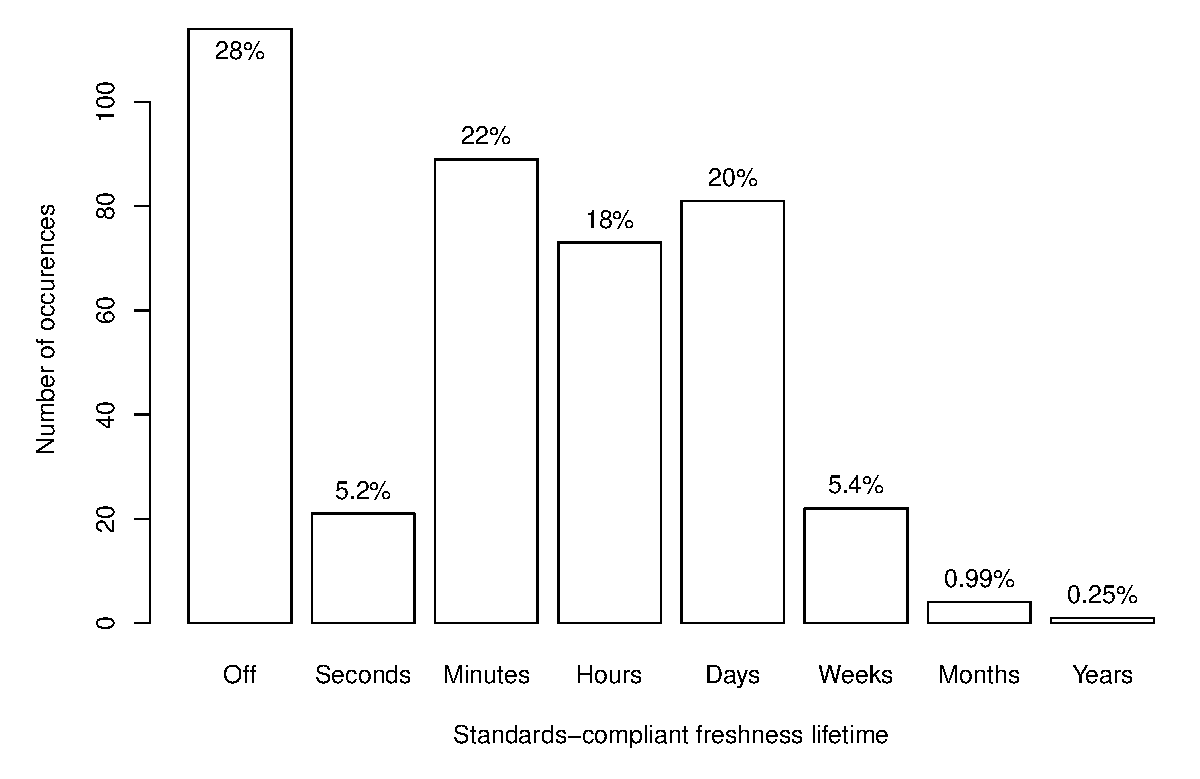
\includegraphics[width=.9\textwidth]{hardall.pdf}}
  \caption{Barplot of all standard-compliant freshness lifetimes
    found. The first bin are the cases where caching is explicitly
    prohibited. The next bins are for lifetimes, where the values are
    grouped if they are on the order of seconds, minutes, hours, etc,
    i.e. the second bin counts the lifetimes in the interval [1,59]
    seconds, etc.}
  \label{fig:hardall}
\end{figure}



In Figure~\ref{fig:hardtable}, we have broken this
up by the type of resource that was accessed, i.e. SPARQL endpoints,
vocabularies, dataset descriptions or unclassified information
resources. First, we note that it seems like the distribution of
freshness lifetime is quite different for the different types, an
observation that is also supported by a similar hypothesis test as
above, with a \pvalue = 0.00001. We also note that it is often
prohibited to cache dataset descriptions. This is odd, since
statistics about datasets is usually costly to compute and should be
cached. The VoID specification \cite{voidnote} also notes that the
statistics are considered estimates.

\begin{figure}[ht]
  \centerline{%
    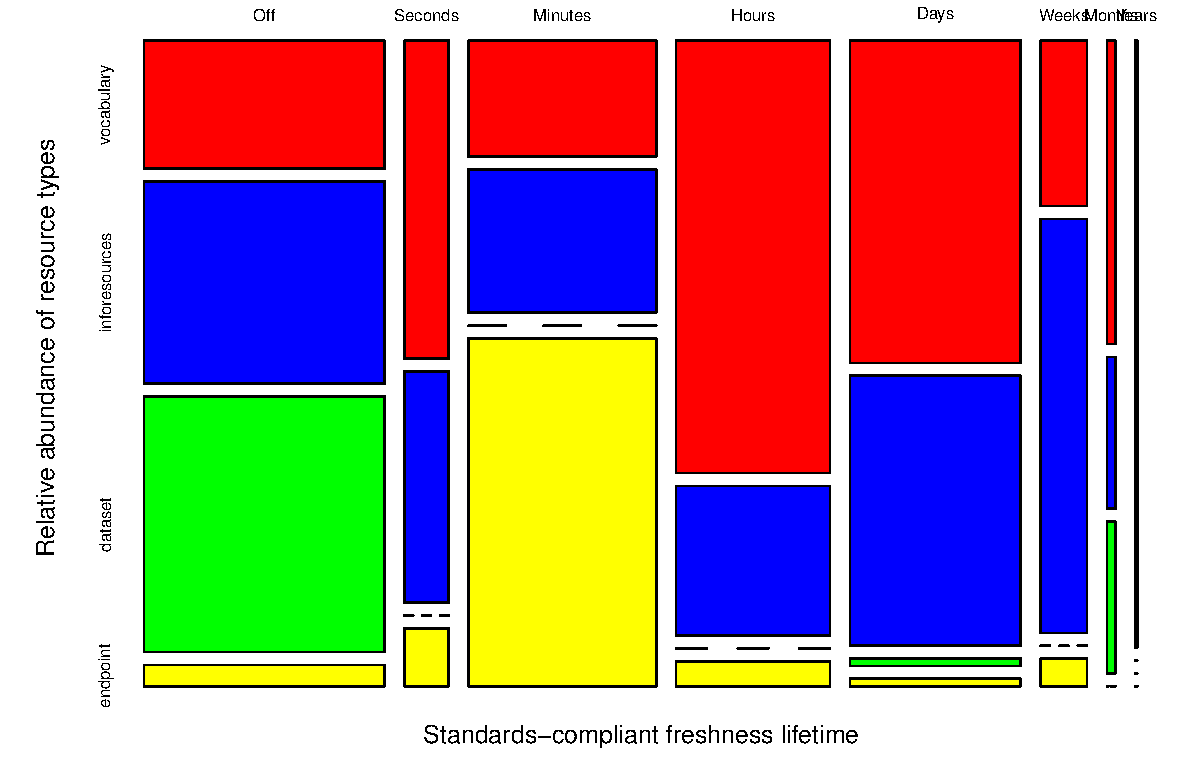
\includegraphics[width=.9\textwidth]{hardtable.pdf}}
  \caption{Mosaic Plot. Divided by type of resource on the vertical
    axis and by the same bins as in Figure~\ref{fig:hardall} on the
    horizontal axis. }
  \label{fig:hardtable}
\end{figure}


We also note that prohibition of SPARQL results caching is rare,
amongst the servers that expose caching headers, it is common
that the result may be cached for some minutes.\todo{more to point
  out?}

\subsubsection{Simple heuristic freshness estimates}\label{sec:simplefresh}

We next consider the simple heuristic freshness lifetime. This is
implemented as suggested in RFC7234, section~4.2.2. This is based on a
fraction of the time lapsed between the current time and the
modification time given in the \httph{Last-Modified} header. This
approach therefore still requires the Web server to be cooperative to
be successful, but commonly, Web servers can track this, based e.g. on
the file modification time of the underlying file system.


\begin{figure}[th!]
  \centerline{%
    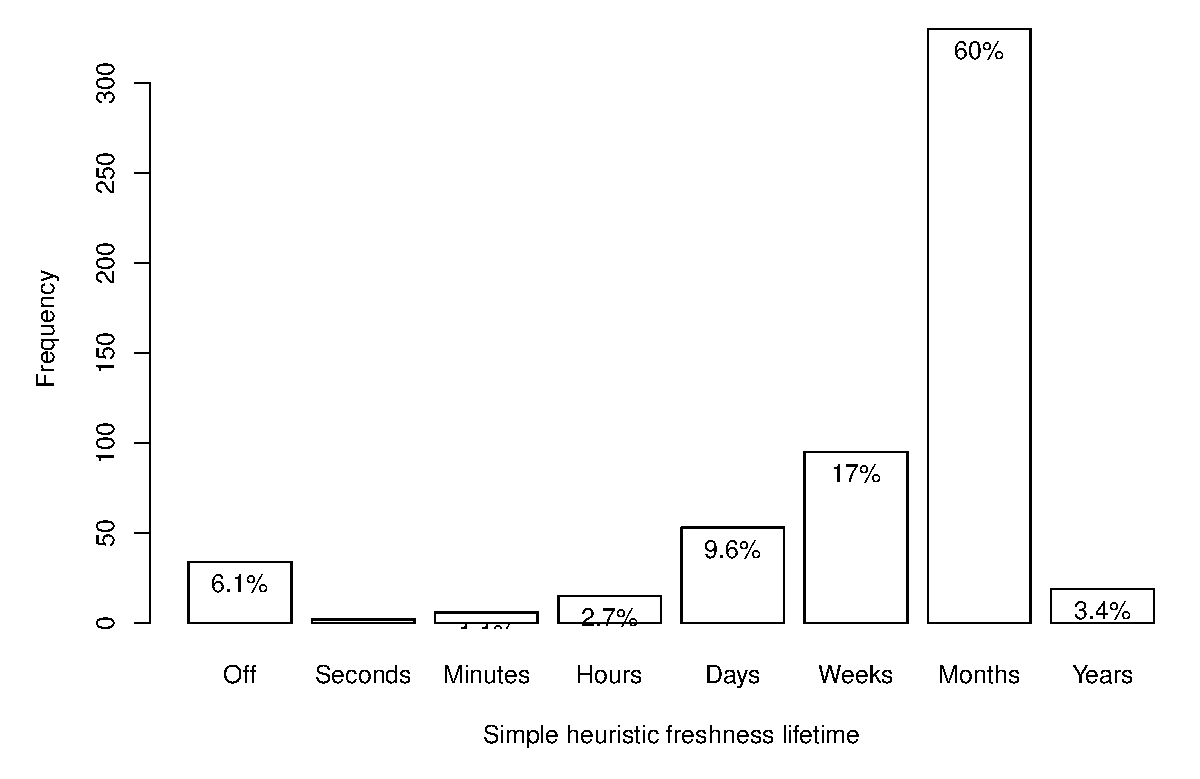
\includegraphics[width=.9\textwidth]{heuristicall.pdf}}
  \caption{Barplot of all simple heuristic freshness lifetimes
    found. Bins as in Figure~\ref{fig:hardall}.}
  \label{fig:heuristicall}
\end{figure}

We were able to compute a heuristic lifetime for 554 resources, a
larger number than standards-compliant resources. In
Figure~\ref{fig:heuristicall}, we see that the distribution of
lifetimes are radically different from the case in
Figure~\ref{fig:hardall}. In this case, we may cache many resources
for months. Only a handful of resources had changed in the last
minutes. Since this is based on actual times since last modifications,
this suggests that many resources should have had explicit cache
headers with very long lifetimes. This is supported by
DyLDO\cite{dyldo2}, which concludes that:
\begin{quote}
[...] We found that 62.2\% of documents didn’t change over the six
months and found that 51.9\% of domains were considered static.
\end{quote}
This agrees well with that 60\% of the simple heuristic lifetimes are
in the month range. 

Moreover, by inspecting Figure~\ref{fig:heuristictable}, we
note that the difference between different types of resources is much
smaller. This is confirmed by a $\chi^2$ test that yields \pvalue =
0.02.

\begin{figure}[hb!]
  \centerline{%
    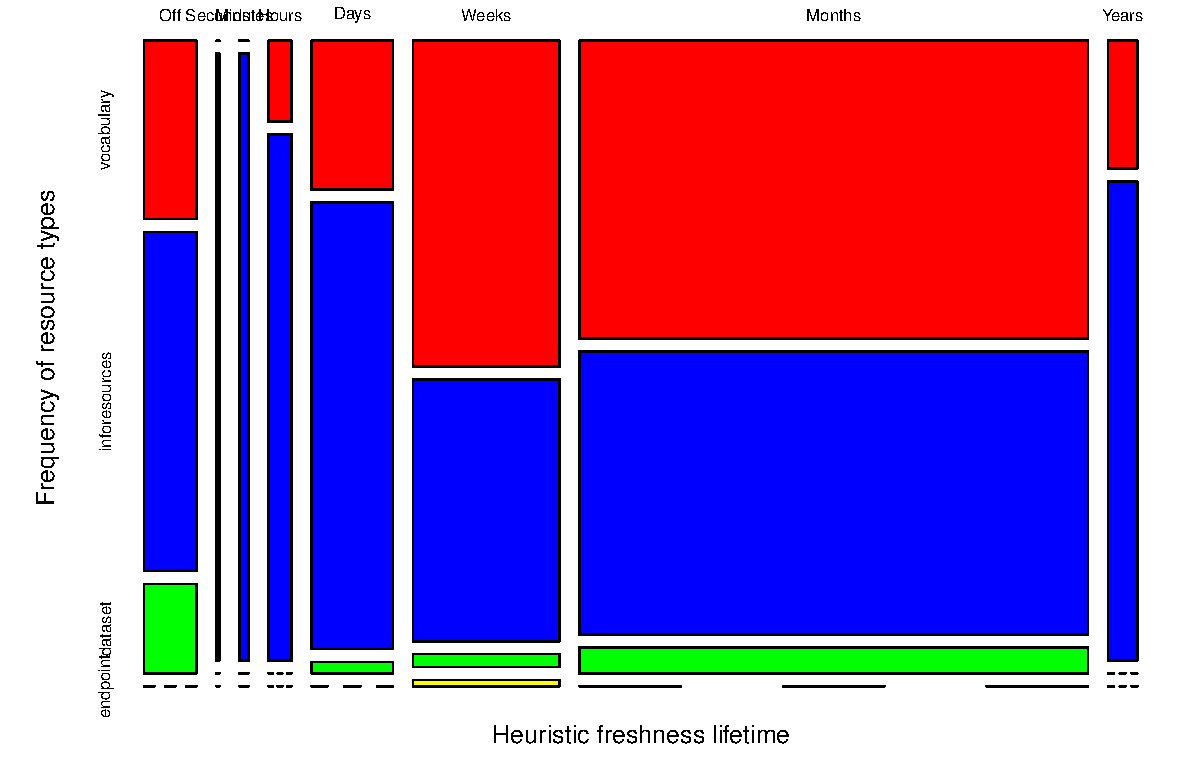
\includegraphics[width=.9\textwidth]{heuristictable.pdf}}
  \caption{Mosaic Plot. Divided by type of resource on the vertical
    axis and by the same bins as in Figure~\ref{fig:hardall} on the
    horizontal axis. }
  \label{fig:heuristictable}
\end{figure}


We find that only one SPARQL Endpoint yields a heuristic lifetime, on
closer inspection, we find this to be hosted by
Dydra\footnote{http://dydra.com/}. We speculate that this is due to
that few underlying DBMS systems help track modification times in a
way that can be used on a SPARQL result basis.

\subsubsection{Heuristic freshness from Dublin Core properties}

We noted that the Dublin Core Metadata terms vocabulary has a number
of predicates that may become useful in determining heuristic
freshness in the future, so we recorded any statements containing the
predicates \rdfterm{dct:date}, \rdfterm{dct:accrualPeriodicity},
\rdfterm{dct:created}, \rdfterm{dct:issued}, \rdfterm{dct:modified} or
\rdfterm{dct:valid}.

First, we compare dates given in \rdfterm{dct:modified} to dates given
in \httph{Last-Modified} when both are available for a resource. They
are often not the same, but it appears that dates in the former are
further back in time than the latter. We speculate that this may be
due to that the webserver tracks semantically insignificant changes
through the filesystem, while authors of RDF only update timestamp
when significant changes are made, or it may be that authors forget to
update their timestamps.

\rdfterm{dct:modified} occurs in 2687 triples, but 2487 of these does
not have the Request-URI of the information resource as their subject,
i.e. it gives the last modification time of some subgraph of the
returned RDF. Nevertheless, given its prevalence, it is highly likely
that the presence of \rdfterm{dct:modified} will be useful in
determining a heuristic freshness lifetime, as the latest date may be
used.\todo{Actually calculate lifetimes based on this and compare}

\rdfterm{dct:valid} occurred 21 times, and could be used in lieu of an
\httph{Expires} header, but none of these occurences had a date in the
future.

\rdfterm{dct:accrualPeriodicity} occurred only twice, and in neither
case contained machine readable data.

\rdfterm{dct:date}, \rdfterm{dct:created} and \rdfterm{dct:issued}
were present in 36, 389 and 1475 triples respectively. They correspond
roughly to the \httph{Date} header, which is present in all requests,
and they are therefore not important, but given their prevalence they
could be useful in further analysis.

\subsection{Cache validation}

Hitherto, we have considered the case where the client or proxy does
not send a HTTP request to the server when a resource that is present
in the cache is requested. This is desireable if the client can be
sufficiently confident that the response is fresh, either by having a
standards-compliant freshness lifetime or a heuristic to determine
it. At the end of this period, or if the previous response had no
lifetime, due to lack of information, or to that the server has stated
so in the \httph{Cache-Control} header, responses must be
revalidated. In this case, RFC7232 defines the behaviour, with
\httph{ETag} and \httph{Last-Modified} as the relevant response
headers.

The BTC had recorded these headers in their data, where 1733 had the
\httph{ETag} header and 690 had \httph{Last-Modified} with a great
overlap. For the resources where either or both were available, we
made our initial request conditional, and 911 responses were verified
as still fresh. 

In total, 1260 successful initial responses contained
an \httph{ETag}, 606 for vocabularies, 117 for datasets, just 12 for
endpoints and 525 for unclassified information resources.

To see if the server actually supported conditional requests, and not
just merely set the response headers, we made another 1822 requests to
the resources that had these headers. Then, we checked if the response
code was 200, and the conditional headers had not changed since our
initial requests. In 85 cases, conditional requests were not supported
according to the standard, no cases for endpoints, 3 for datasets and
23 for vocabularies, 59 for generic information resources.\todo{table instead?}


We already used \httph{Last-Modified} to compute heuristic lifetime
in Section~\ref{sec:simplefresh} for 554 resources.\todo{really needed?}



\section{Future work}

Identify implementations that expose suitable caching headers.

Investigate whether curated collections such as LOV or SPARQLES
contain resources that has different characteristics. Since the
different sources we surveyed overlap, this cannot be done with
Pearson's $\chi^2$ test, but requires more sophisticated statistics.

Monitor the change frequency and use a contingency table to assess the
correctness of caching headers.

Further investigate the correctness of the \rdfterm{dct:modified} property.

\section{Recommendations}\todo{write}

Based on the results of DyLDO, it is highly likely that most cache
prohibitions are misguided, and server administrators are adviced to
turn them off unless they are sure they are required.

Data owners should seek to understand their change frequency, and
adjust cache headers accordingly. Framework authors should make it
easy to set the expected lifetime, and manage changes to the
publishing schedule.

To allow generation and validation of \httph{Last-Modified} and
\httph{ETag} headers, DBMS authors should make sure it is much cheaper
to retrieve the modification time of any subgraph, than to retrieve
the subgraph itself. This would be a great improvement for
RFC7232-based caching, when revalidation is required. It would also
help simple heuristic based caching. Research in that direction has
been published in \cite{kaseicache}.

A change periodicity predicate should be standardized in Void.

All Web cache implementations we have studied have cached responses in
the form of a key that identifies a serialized object. For short-term
impact, future work should accept this as an architectural constraint.

\bibliographystyle{plain}
%\bibliographystyle{abbrv}
%\bibliographystyle{jbact}
%\bibliographystyle{splncs03}
\bibliography{webarch,data,rfc,hypermedia,dynamicity,stat1,specs,vocabs}


\begin{subappendices}
\renewcommand{\thesection}{\Alph{section}}%

\section{Implementation of data reduction}\label{app:reduction}

The Billion Triple Challenge 2014 dataset provided data in the form of
NQuad files. Due to the presence of invalid RDF, we iterated through
the NQuad files on a line-by-line basis. First, we matched each line
against a regular expression were lines matching
\texttt{ontology|endpoint|sparql|vocabular} passed the filter. Then,
the Perl framework
RDF::Trine\footnote{https://metacpan.org/release/GWILLIAMS/RDF-Trine-1.011} was used
to parse the line. Lines that failed to parse was discarded. We have
not investigated whether this could introduce biases. Statements were
then accepted into a new NQuad file if they had a predicate that
matched the
\rdfterm{sd:endpoint}\footnote{http://www.w3.org/TR/sparql11-service-description/\#sd-endpoint}
or matched a case-insensitive regular expression \texttt{sparql} if
the subject and objects were both resources, or the predicates
\rdfterm{void:vocabulary}\footnote{http://www.w3.org/TR/void/\#vocabularies},
\rdfterm{rdfa:vocabulary}\footnote{http://www.w3.org/TR/rdfa-core/\#term-prefix-definitions-vocabulary}
or
\rdfterm{api:vocabulary}\footnote{http://purl.org/linked-data/api/vocab\#vocabulary},
as well as having an resource as object. Finally, statements with the
the classes
\rdfterm{cogs:Endpoint}\footnote{http://vocab.deri.ie/cogs\#Endpoint},
\rdfterm{owl:Ontology} and
\rdfterm{voaf:Vocabulary}\footnote{http://lov.okfn.org/vocab/voaf/v2.3/index.html\#Vocabulary}
in the object position were also accepted. More classes and properties
were considered, but not used in the data reduction if they did not
occur in the original data.

In the next step, we filtered out statements with URIs that were
invalid or irrelevant, e.g. URIs that didn't have a scheme or where
the scheme wasn't HTTP(S), or they were referring to private IP addresses.

We then sought to classify resources into the categories ``endpoint''
for SPARQL endpoints, ``vocabulary'' for ontologies, ``dataset'' for
datasets that may contain further descriptions of several resources,
or simply ``inforesources'' for those that did not fit in the above
classes. To do so, we classified based on certain predicates and
classes, see table\todo{create table}. Additionally, URIs derived from
prefix.cc were classified as ``vocabulary'' and those from SPARQLES as
``endpoint''.

Since we blatantly violated URI opacity with our regular expression
matching in the first step, we needed to further filter candidates for
SPARQL endpoints. This step therefore included filtering as well as
classification.

We found in the data a large number of ontologies that consist of many
information resources with just a few triples in each. Since they
appear to be produced by the same software, usually Semantic
Mediawiki, we assume that they are configured with a single setup, and
thus we will merely sample these resources.

We continued to also sample the HTTP headers gathered in the BTC2014
dataset. 
%as they had recorded some of the relevant headers,
%\httph{Expires}, \httph{Last-Modified} and \httph{ETag}. 
First, we traversed the files with a simple UNIX \texttt{grep} to find
the resources that had reported one of the RDF serializations as
content type. We then traversed this list, first discarded the
resources that did not have a valid IRI (this amounted to just 3273
resources). For the resources we found, as well as for the resources
that was of \rdfterm{rdf:type owl:Ontology} above, we kept one
resource per hostname, with the exception of the popular blogging
platforms Livejournal and SAPO, where each blog has their own host and
they expose FOAF data. For those, we only kept one hostname. 

\section{Implementation of spider}\label{app:fetcher}

We then developed a fairly elaborate parallel spider to examine the
resources found on hosts that the previous steps deemed interesting
using the Perl frameworks RDF::Trine and libwww. The spider operated
with a timeout of 20 seconds and a maximum message size it would
accept of 1 MB.

The parallel spider would then launch a process per host, but each
request to one host would be delayed by 10 seconds. For each host, the
spider would go through the list of URLs found by previous steps for
that host. Since the BTC2014 recorded
the \httph{Expires} (an RFC7234 caching header), \httph{Last-Modified}
and \httph{ETag} (RFC7232 conditional request) headers where they
existed, we first examined if any of the resources were still fresh,
but none were. Wherever the last two headers existed, we added the
corresponding \httph{If-Modified-Since} and \httph{If-None-Match}
headers for a conditional initial request.

\begin{table}
\caption{Recorded HTTP headers}\label{tab:headers}
 \begin{tabular}{ | l |  p{3cm} | p{5cm} |}
    \hline
    Header & Reference & Description \\ \hline
\httph{Age} & RFC7234 & When obtaining response from a cache, the number of
seconds since validation \\ \hline
\httph{Cache-Control} & RFC7234 & Header used for a variety of directives \\ \hline
\httph{Expires} & RFC7234  & Gives the date/time after which the
   response is considered stale. \\ \hline
\httph{Pragma} & RFC7234 & Archaic HTTP 1.0 header  \\ \hline
\httph{Warning} & RFC7234  & For additional information about possible incorrectness \\ \hline
\httph{Content-Type} & RFC7231 & To select the correct parser \\ \hline
\httph{If-None-Match} & RFC7232  & Request header to check if
                                   \httph{ETag} has changed   \\ \hline
\httph{If-Modified-Since} & RFC7232  & Request header to check if
                                   \httph{Last-Modified} has changed    \\ \hline
\httph{Last-Modified} & RFC7232 & When the resource was last modified \\ \hline
\httph{ETag} & RFC7232 & An opaque validator to check if the resource
has changed  \\ \hline
\httph{X-Cache} &  & Inserted by some caches to indicate cache status \\ \hline
\httph{Date} & RFC7231 & The time of the message. Used in conditional requests
and heuristics \\ \hline
\httph{Surrogates} & Edge Architecture Specification\cite{edgearch} & Draft
to allow more fine-grained control for proxies. \\ \hline
\httph{Client-Aborted} & libwww\footnote{https://metacpan.org/release/GAAS/libwww-perl-6.04}  & Header inserted by User
Agent to indicate that it aborted the download \\ \hline
\httph{Client-Warning} & libwww  & Header inserted by User
Agent to give details about problems with the download \\ \hline

    \hline
    \end{tabular}
\end{table}


For endpoints, we made the following SPARQL query:
\begin{verbatim}
SELECT DISTINCT ?Concept WHERE {[] a ?Concept} LIMIT 2
\end{verbatim}
which should be quite light, yet likely yield results.

Then, the first request would be made, and a selection of the
resulting HTTP headers recorded in an per-host NQuads file. For this
purpose, we developed and released a module
RDF::Generator::HTTP\footnote{https://metacpan.org/release/KJETILK/RDF-Generator-HTTP-0.003}
to the Comprehensive Perl Archive Network. We recorded whether the
conditional request showed that the BTC data were still fresh, and if
it was, we retrieved the current data, as we had not couple the
headers to the body in our original retrieval.

Based on the resulting headers, we first let libwww calculate the
freshness lifetime in seconds if it was possible, and recorded
that. Then, we also let it calculate a \emph{heuristic} freshness
time based on a suggestion in RFC7234, section~4.2.2, and recorded that.

If the initial response had RFC7232 headers, we make another
request to see if the server just included the headers but does not
actually support conditional requests. The heuristic we employed is
that if the headers remain the same, but the result was returned,
rather than just a response code \httph{304} (which indicates that the
previous result can be reused), then the server does most probably not
support it.

For endpoints, we examined the response message, to see if there are
any results to our query, and recorded that if there are. In addition
to the endpoints registered in the SPARQLES survey, our process found
18~endpoints that responded with results.

For all others, we parsed the response, and recorded any errors if the
parser concluded the content were invalid.

For resource types other than ``vocabulary'', we look for SPARQL
endpoints in the response, using the predicates \rdfterm{sd:endpoint}
and \rdfterm{void:sparqlEndpoint}. We then do the same query as above
and record the relevant headers. Unfortunately, we found early that
this only turns up misconfigured endpoints that point to localhost,
and was removed from the spider for the final analysis.

Finally, if the LOV SPARQL endpoint used a URI for the vocabulary that
was different from the namespace URI (after a normalization step),
another request would be made to record the selected HTTP headers from
that as well.\todo{say how many requests failed? It was a lot}
\end{subappendices}



\end{document}
